\documentclass[12pt]{beamer}
\usetheme[
%%% option passed to the outer theme
%    progressstyle=fixedCircCnt,   % fixedCircCnt, movingCircCnt (moving is deault)
  ]{Feather}

% If you want to change the colors of the various elements in the theme, edit and uncomment the following lines

% Change the bar colors:
%\setbeamercolor{Feather}{fg=red!20,bg=red}

% Change the color of the structural elements:
%\setbeamercolor{structure}{fg=red}

% Change the frame title text color:
%\setbeamercolor{frametitle}{fg=blue}

% Change the normal text color background:
%\setbeamercolor{normal text}{fg=black,bg=gray!10}

%-------------------------------------------------------
% INCLUDE PACKAGES
%-------------------------------------------------------

\usepackage[utf8]{inputenc}
\usepackage[english]{babel}
\usepackage[T1]{fontenc}
\usepackage{helvet}

%-------------------------------------------------------
% DEFFINING AND REDEFINING COMMANDS
%-------------------------------------------------------

% colored hyperlinks
\newcommand{\chref}[2]{
  \href{#1}{{\usebeamercolor[bg]{Feather}#2}}
}

%-------------------------------------------------------
% INFORMATION IN THE TITLE PAGE
%-------------------------------------------------------

\title[] % [] is optional - is placed on the bottom of the sidebar on every slide
{ % is placed on the title page
	  \textbf{Mining and Analysis}
}

\subtitle[The Feather Beamer Theme]
{
	  of \textbf{Courses} and \textbf{Students} Data \\ about the \textbf{Computer Science Degree}
}

\author[Simone Cipriani]
{      \textbf{Simone Cipriani} \\
	   \textit{prof.} \textbf{Donatella Merlini}
}

\institute[]
{
	  Scuola di Scienze Matematiche, Fisiche e Naturali\\
	  Università degli Studi di Firenze\\

  %there must be an empty line above this line - otherwise some unwanted space is added between the university and the country (I do not know why;( )
}

\date{\today}

%-------------------------------------------------------
% THE BODY OF THE PRESENTATION
%-------------------------------------------------------

\begin{document}

%-------------------------------------------------------
% THE TITLEPAGE
%-------------------------------------------------------

{\1% % this is the name of the PDF file for the background
\begin{frame}[plain,noframenumbering] % the plain option removes the header from the title page, noframenumbering removes the numbering of this frame only
  \titlepage % call the title page information from above
\end{frame}}

%-------------------------------------------------------
% SLIDES
%-------------------------------------------------------

%-------------------------------------------------------
\begin{frame}{Introduction}{A general view about the Data Mining process}
%-------------------------------------------------------
	\begin{centering}
		\vspace{0.2cm}
		\hspace{-0.2cm}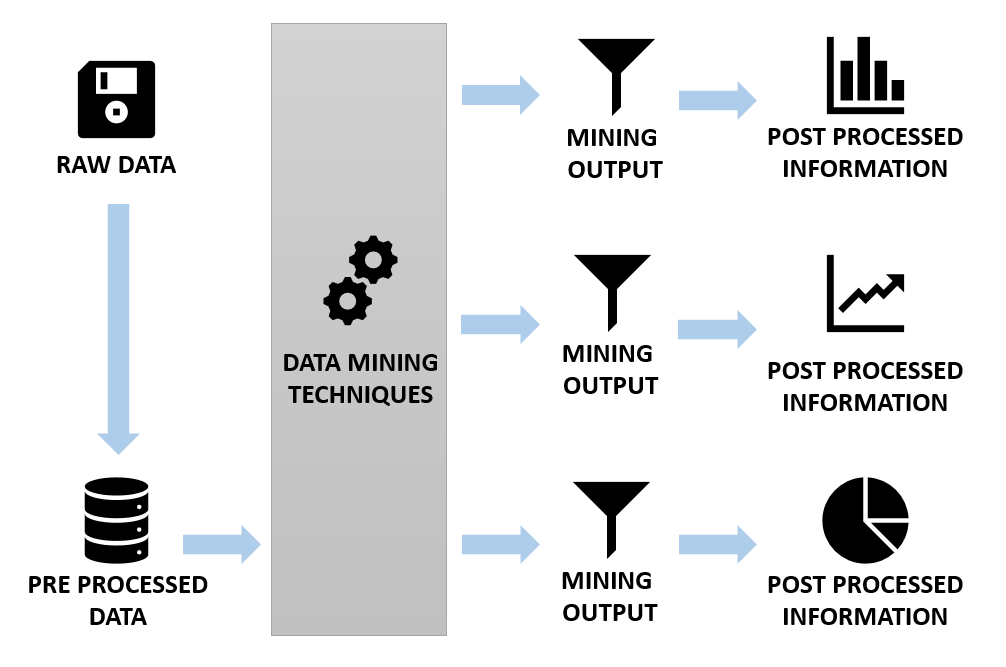
\includegraphics[scale=0.25]{img1_noback.png}
	\end{centering}
\end{frame}

%-------------------------------------------------------
\begin{frame}{Introduction}{The choice of appropriate technologies: picking the right tools}
%-------------------------------------------------------

	\begin{block}{}
	    \begin{itemize}
		    \item<1-> \alert{Data Processing}: \hspace{0.2cm} 
\includegraphics[scale=0.18, trim=0 0.8cm 0 0]{../thesis/img/mongodb.png} \\\vspace{0.2cm} \emph{New tech, noSQL paradigm, \textcolor{cyan}{good skill to learn!}}
		    \item<2-> \alert{Data Mining Algorithms}: \hspace{0.2cm} 
\includegraphics[scale=0.16, trim=0 3.2cm 0 0]{../thesis/img/weka_noback.png}  \\\vspace{0.35cm} \emph{Open source data mining software/framework;} \\\vspace{0.2cm}
			\item<3-> \alert{Visualization Techniques}: \hspace{0.2cm} 
\includegraphics[scale=0.18, trim=0 2cm 0 0]{../thesis/img/R.png} \hspace{0.4cm} 
\includegraphics[scale=0.012, trim=0 25cm 0 0]{excel.png} \\\vspace{0.35cm} \emph{R is powerful, but spreadsheets are easier to use.}
	    \end{itemize}
    \end{block}

\end{frame}

%-------------------------------------------------------
\begin{frame}{Raw Data}{What is the nature of the raw material? How can we use it?}
%-------------------------------------------------------

\begin{itemize}

    \item<1->\textbf{Data about \alert{students}}: \emph{anonymous students records} about academic career results, in a certain time span: \\
        \noindent\begin{centering}
            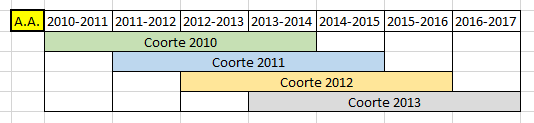
\includegraphics[scale=0.50]{../raw/stud_comp.png}
        \end{centering}

    \vspace{0.2cm}

    \item<2->\textbf{Data about \alert{courses}}: teachings evaluations questionaries compiled by the students, in an \emph{aggregate form}, about those Academical Years: \\ \vspace{0.1cm}
        \hspace{0.6cm}\textcolor{cyan}{\texttt{2010-2011, 2011-2012, \ldots, 2016-2017}}

\end{itemize}

\end{frame}

%-------------------------------------------------------
\begin{frame}{Students Data Understanding}{Example of visualization technique: interpreting a scatter plot}

    \vspace{0.2cm}
    \begin{centering}
        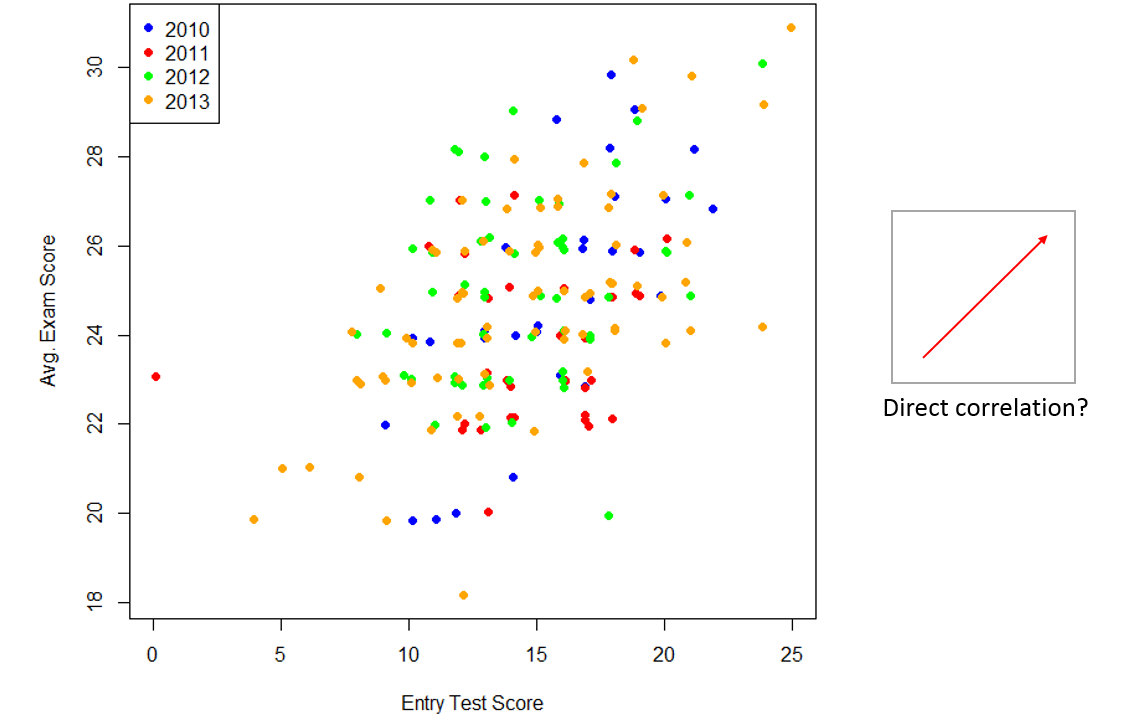
\includegraphics[scale=0.28]{img2_noback.png}
    \end{centering}

\end{frame}

\begin{frame}{Students Data Understanding}{Interpreting a std. dev. matrix about first year exam scores}

    \vspace{0.25cm}
    \noindent\begin{centering}
        \hspace{-1cm}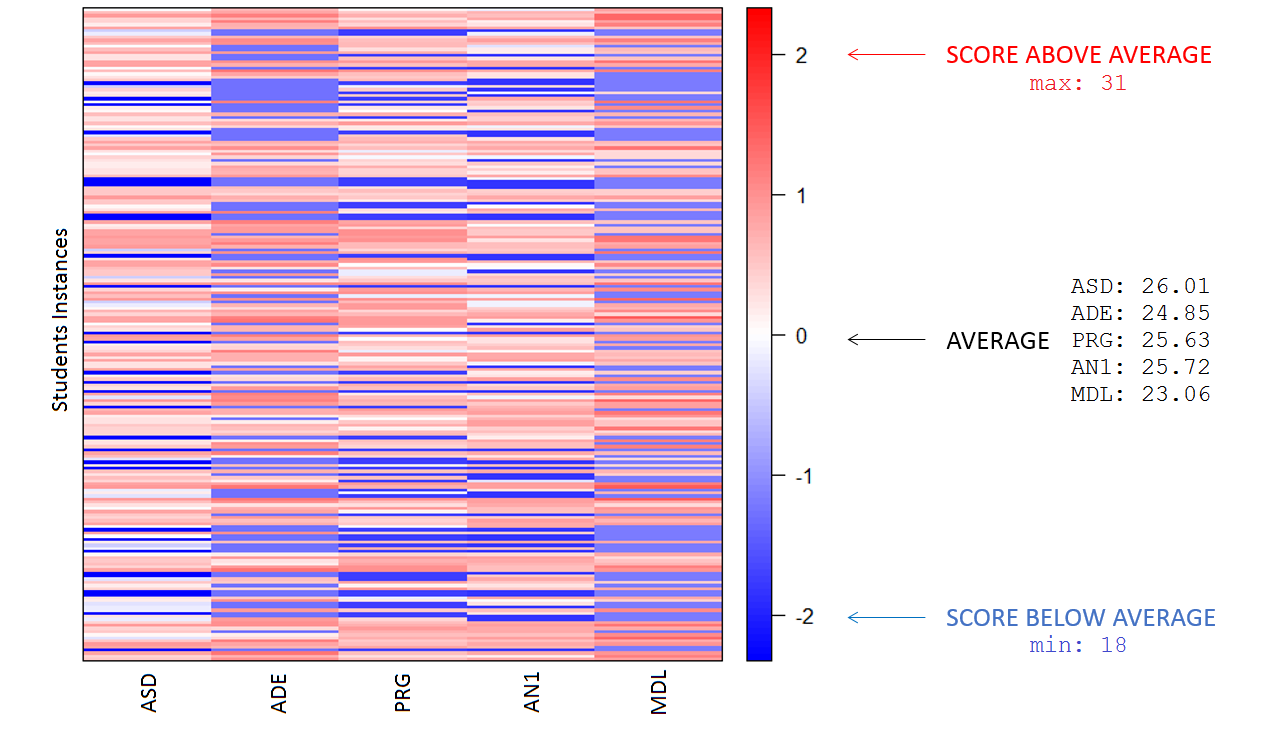
\includegraphics[scale=0.38]{img3.png}
    \end{centering}

\end{frame}

\begin{frame}{Preprocessing}{How can we combine all the available data in a single set?}

\vspace{0.15cm}

    \emph{Raw} data sets has to be \textcolor{cyan}{cleaned}, and \emph{disaggregated data} can be \textcolor{cyan}{aggregated} to match the appropriate \emph{primary key}. \\

    \vspace{0.25cm}

    Then, they can be \alert{joined} --- for example, like this:

    \vspace{0.25cm}

    \begin{centering}
        \hspace*{-0.65cm}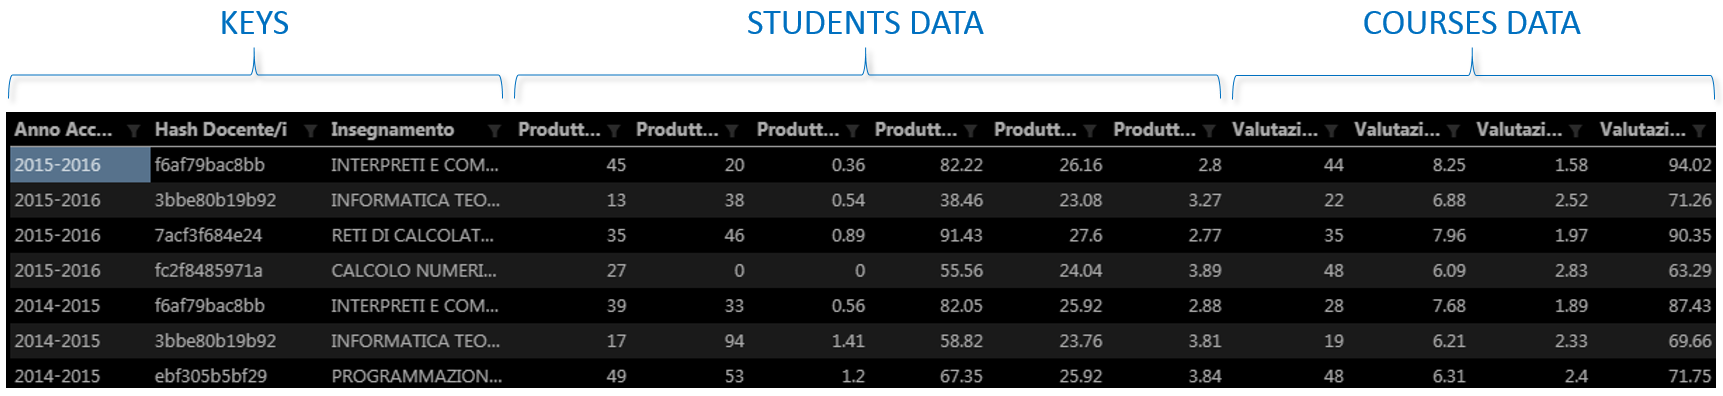
\includegraphics[scale=0.2]{prepr2.png}
    \end{centering}

\vspace{-0.35cm}
    Before attemping any data mining technique, data may still need \textcolor{cyan}{discretization}, \textcolor{cyan}{normalization}, etc. \\

 \vspace{0.25cm}

    Each analysis needs its own \emph{specific preprocessing}.

\end{frame}
\begin{frame}{Cluster Analysis}{How can we find semantic groups among data instances?}

\vspace{0.1cm}
\centering{How can we obtain a clustering on the joined data set?} \vspace{0,3cm}
\vspace{-0.2cm}
	\begin{block}{}
		\begin{itemize}
			\item<1-> \alert{K-Means} --- Others algorithms as been tried, but K-Means gave the best results; \vspace{0.2cm}
            \item<2-> \alert{Euclidean distance metric} --- Straight line distance between two points in an Euclidean Space; \vspace{0.2cm}
			\item<3-> \alert{Looking for 2 clusters} --- Deviding teaching courses instances in \textcolor{cyan}{\emph{good}} ones and \textcolor{cyan}{\emph{not-so-good}} ones; \vspace{0.2cm}
			\item<4-> \alert{Considering 3 attributes} --- Each one express a fundamental aspect of the whole data set: \textcolor{cyan}{\emph{average exam score}}, \textcolor{cyan}{\emph{average teaching evaluation}} and \textcolor{cyan}{\emph{average delay}}.
		\end{itemize}
	\end{block}

\end{frame}

\begin{frame}{Cluster Analysis}{How can we obtain a clustering on the joined data?}

\vspace{0.2cm}
\begin{columns}
\begin{column}{0.5\textwidth}
   \textcolor{cyan}{Section} of the data space:
\end{column}
\begin{column}{0.5\textwidth}
     \textbf{X axis}: \emph{average delay} \\ \textbf{Y axis}: \emph{average exams mark}
\end{column}
\end{columns}

    \vspace{0.1cm}
    \begin{centering}
        \hspace{0.5cm}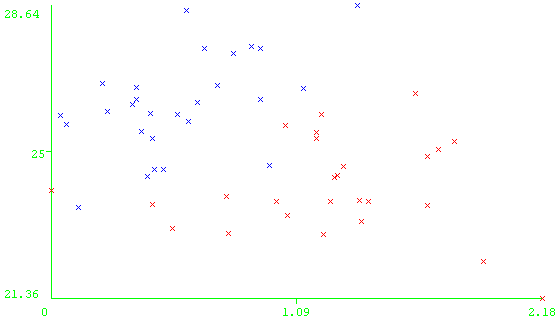
\includegraphics[scale=0.64]{cluster1.png}
    \end{centering}

    \textcolor{blue}{Cluster 0}: good courses --- \textcolor{red}{Cluster 1}: bad courses

\end{frame}

\begin{frame}{Cluster Analysis}{How can we evaluate the obtained clustering?}

\vspace{0.3cm}
\begin{centering}
    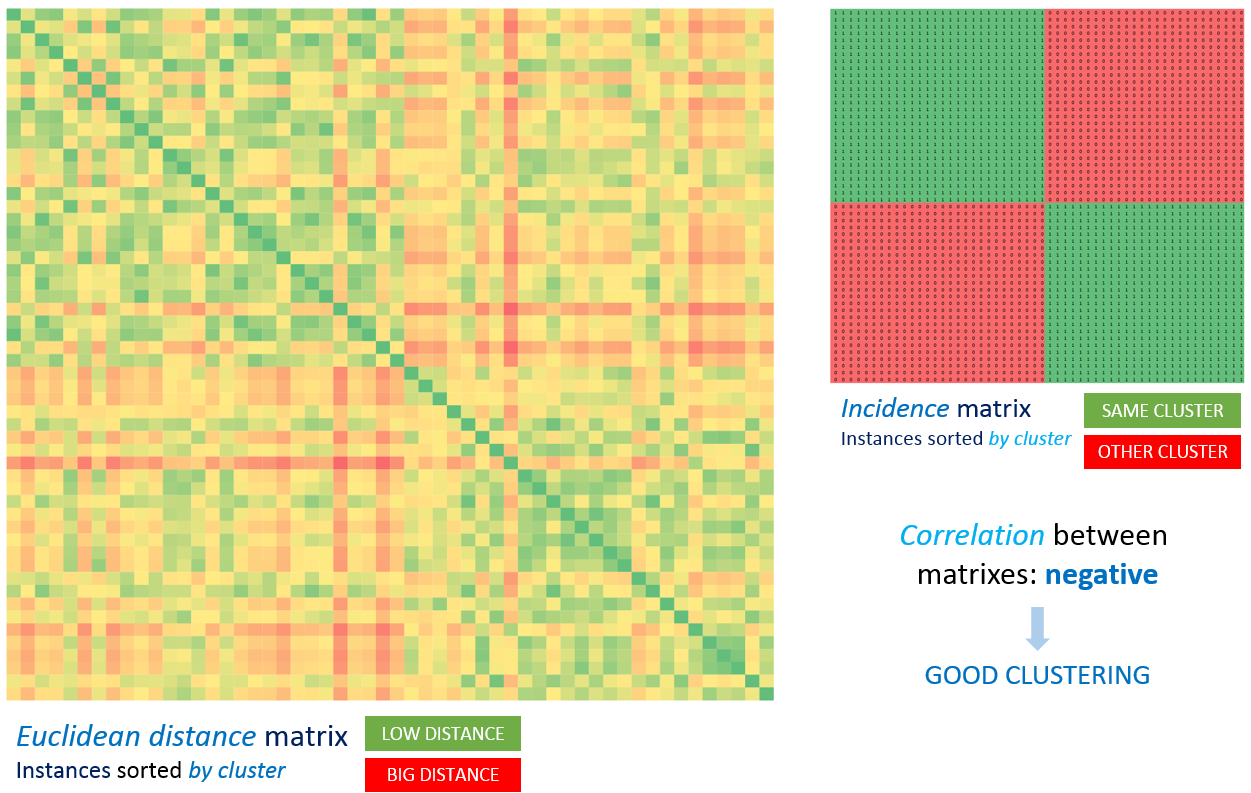
\includegraphics[scale=0.25]{cluster5_nocorr.png}
\end{centering}

\end{frame}

\begin{frame}{Cluster Analysis}{Cluster's composition: analysis and interpretation}

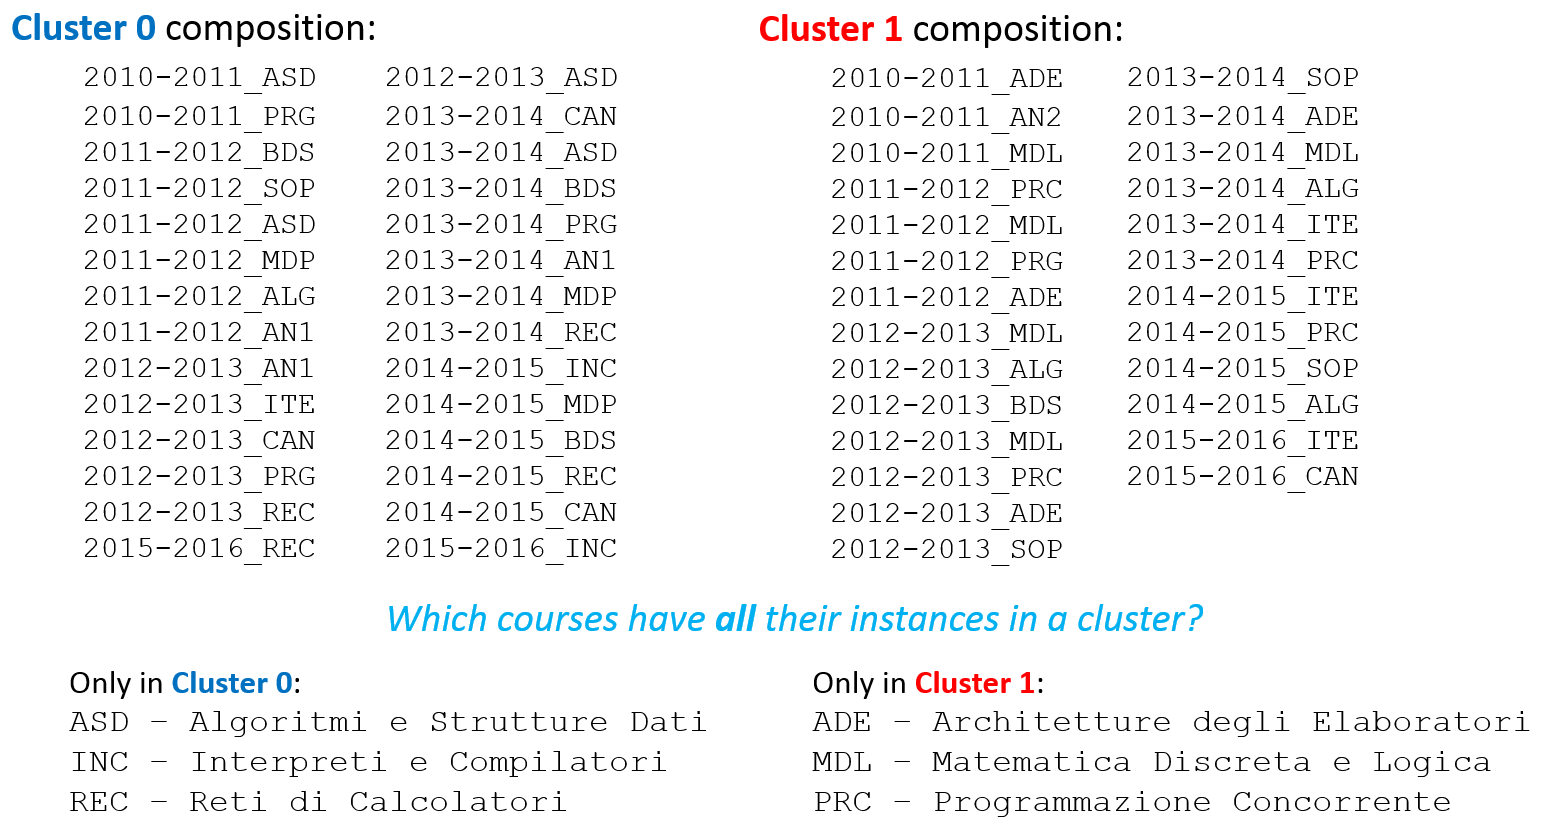
\includegraphics[scale=0.22, trim=2.2cm 0 0 0]{cluster6.png}

\end{frame}

\begin{frame}{Associative Rules Analysis}{Looking for implications among the dataset's attributes}
\vspace{0,2cm}
\centering{What do we need to perform an associative analysis?} \vspace{0,2cm}

	\begin{block}{}
		\begin{itemize}
			\item<1-> \alert{Apriori algorithm} --- it uses an heuristic technique to render the \emph{candidate generation problem} computable;\vspace{0.2cm}
			\item<2-> \alert{Confidence metric} --- a good one is \textcolor{cyan}{lift}, as it values a rule ability to predict cases comparing it against the odds of a random prediction.
            \item<3-> \alert{Discretization} --- we need \emph{discrete attributes} in order to find logical implications between them;\vspace{0.2cm}
            \item<4-> \alert{Focus on a few attributes} --- the same ones chosen for clustering will do: \textcolor{cyan}{\emph{exam score}, \textcolor{cyan}{\emph{delay} and \textcolor{cyan}{teaching evaluation}}}.
		\end{itemize}
	\end{block}

\end{frame}

\begin{frame}{Associative Rules Analysis}{Looking for implications among the dataset's attributes: results}

\vspace{1mm}
\noindent\hspace{-5mm}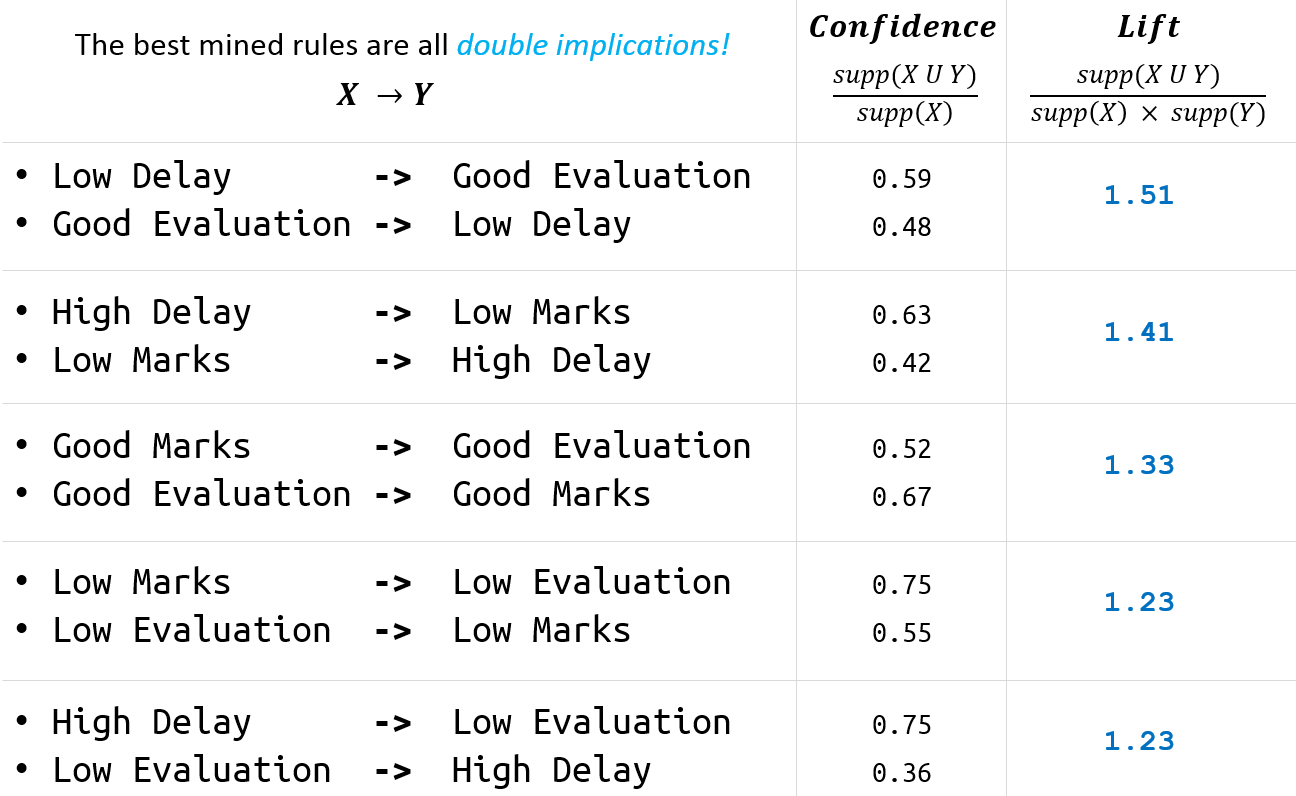
\includegraphics[scale=0.26]{ass6.png}

\end{frame}

\begin{frame}{Frequent Sequential Patterns}{Looking for meaningful frequent patterns in exams sequences}

    \centering\textit{Which exams are \textcolor{cyan}{skipped} the most by the students?} \vspace{0,3cm}

\begin{block}{Mining process}
		\begin{itemize}
			\item<1-> \alert{GSP algorithm} --- Apriori-based algorithm to extract frequent sequential patterns from the \emph{students} data; \vspace{0.2cm}
			\item<2-> \alert{Unusual pattern mining} --- filtering of the GSP output, with the goal of discarding uninteresting (regular) exams patterns; \vspace{0.2cm}
			\item<3-> \alert{Out-of-place exams mining} --- extraction of the exams that are passed \emph{after} a later exam.
		\end{itemize}
	\end{block}

\end{frame}

\begin{frame}{Associative Rules Analysis}{Looking for implications among the dataset's attributes}
\vspace{0.3cm}
\begin{columns}
\begin{column}{0.5\textwidth}
    \hspace{0.6cm}Exams \textcolor{cyan}{right order}:\\
    \vspace*{0.3cm}
    \hspace*{0.2cm}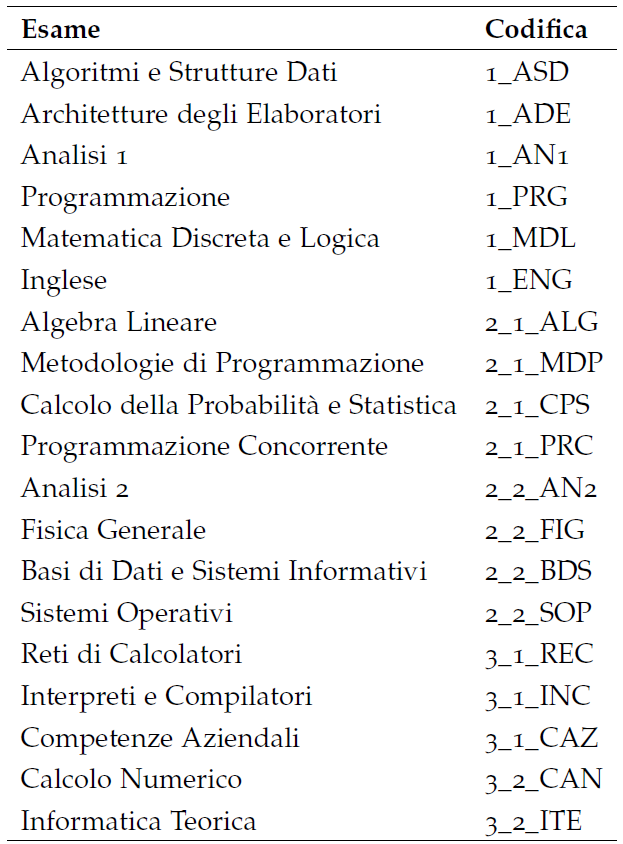
\includegraphics[scale=0.20]{seq1.png}
\end{column}
\begin{column}{0.5\textwidth}
    \hspace*{-0.5cm}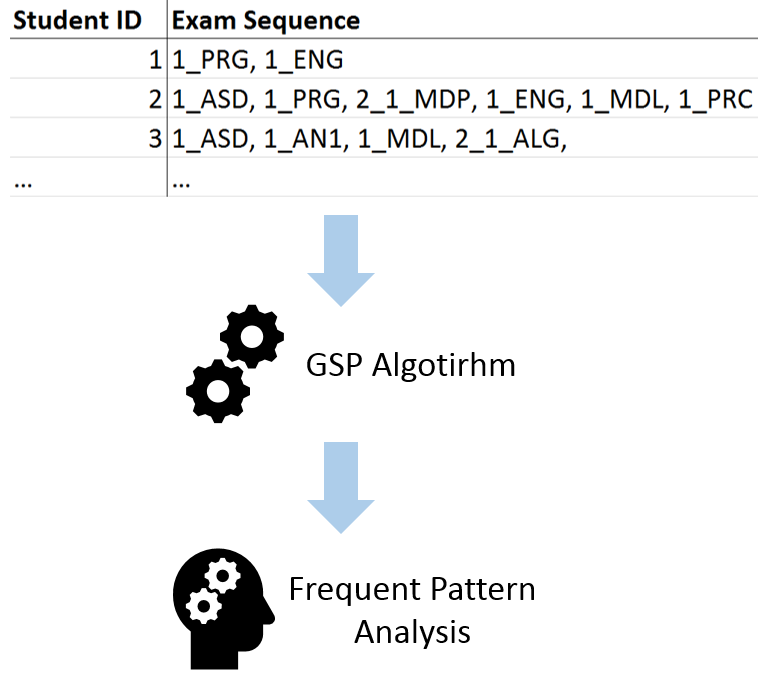
\includegraphics[scale=0.21]{seq3.png}
\end{column}
\end{columns}

\end{frame}

\begin{frame}{Associative Rules Analysis}{Looking for implications among the dataset's attributes}

    \alert{Example} of a \textcolor{cyan}{frequent}, \textcolor{cyan}{unusual} pattern: \\

	\vspace{0.3cm}
	\begin{centering}
		\texttt{3\_2\_CN, 3\_2\_ITE, 2\_2\_FIG}\\
	\end{centering}
	\vspace{0.3cm}

	\ldots which stands for:

	\vspace{0.3cm}
	\begin{centering}
	\texttt{Calcolo Numerico, Informatica Teorica, Fisica Generale}\\
	\end{centering}
	\vspace{0.6cm}

	\texttt{Fisica Generale} is \alert{out of place}, for it is a $2^{nd}$ year exam done after some $3^r{d}$ year exams.\\

\end{frame}

\begin{frame}{Associative Rules Analysis}{Looking for implications among the dataset's attributes}

\vspace{0.1cm}
	Counting how many times an exams is out of place and making proportions with all out-of-place exams, we get...\\ \vspace{0.2cm}

    \begin{centering}
        \hspace*{2cm}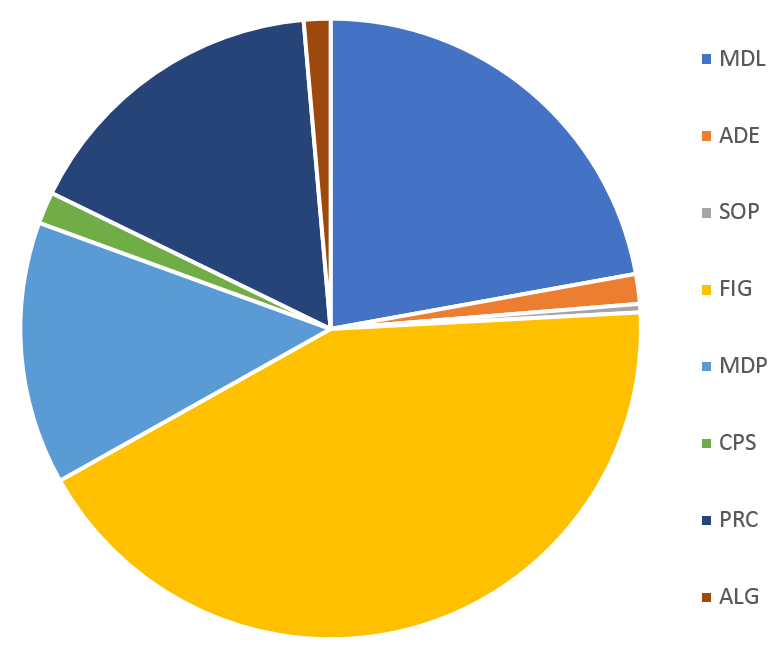
\includegraphics[scale=0.25]{seq2.png}
    \end{centering}

\end{frame}

{\1
\begin{frame}[plain,noframenumbering]
  \finalpage{That's all!\\ \ldots but we only scratched the surface\ldots \\ \vspace{5mm}
  Thank you for your time.}
\end{frame}}

\end{document}